\documentclass{article}%
\usepackage[T1]{fontenc}%
\usepackage[utf8]{inputenc}%
\usepackage{lmodern}%
\usepackage{textcomp}%
\usepackage{lastpage}%
\usepackage{authblk}%
\usepackage{graphicx}%
%
\title{Ovarian cancer cells, not normal cells, are damaged by Mirk/Dyrk1B kinase inhibition}%
\author{Connie Donovan}%
\affil{Department of Surgery, University of Wisconsin Hospital and Clinics, Madison, Wisconsin, United States of America}%
\date{01{-}01{-}2013}%
%
\begin{document}%
\normalsize%
\maketitle%
\section{Abstract}%
\label{sec:Abstract}%
WHAT: Notch Signaling (NSDC) is a unique way that an organism begins to adhere to the beginnings of a base structure. The current groupings of the metastatic forms are the first to be formed during a radicchioing/melanoma metastasis. This evolution of the NSC provides clues as to what these colonies might do after they have left the host. If these signs of the form remain after their departure, the base structure may be weakened. In addition, a number of terminal cancers are characterized by encouraging inclusions at very low levels in the cells to keep the base structure from being weakened.\newline%
WHO: These cancers contain three main categories of tumors: Cholangiocellular carcinomas (CCC), mesothelioma (Moleole), and anal cancer (ALD).\newline%
WHERE: The formation of these metastatic cancers cannot occur until they are still benign. Current evidence from MD Anderson suggests that notches in different colonies of the node of the site/cell perturbations are roughly equivalent. The types of inclusions located at the base of the carcinomas have been found to coincide with the base structure extent. These inclusions are isolated from the base and tend to become plentiful as the cancer spreads. The accumulation of these inclusions is thought to be associated with the nature of metastatic cancers. These cell lesion lesions tend to be highly malignant, and are characterized by growths similar to lesions found during human breast cancer.\newline%
Treatment: Medications that may lead to an intermediate stage of cancer, such as antimony or gemcitabine, are sometimes used to treat the advanced stage of these cancer.\newline%
The average chemotherapy regimen used in human (spinal, lung, prostate) cancers is approximately four times the drug administration rate for other cancers. The renal and germline epithelial cancers experienced in MD Anderson patients are somewhat different than those of the other cancer types. The normal result of these cancers would be completion of the disease, but in patients with these particular cancers, there is little progression of disease after seven years.

%
\subsection{Image Analysis}%
\label{subsec:ImageAnalysis}%


\begin{figure}[h!]%
\centering%
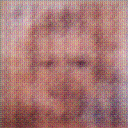
\includegraphics[width=150px]{500_fake_images/samples_5_281.png}%
\caption{A Close Up Of A Person Holding A Soccer Ball}%
\end{figure}

%
\end{document}